% Author: Dr. Matthias Jung, DL9MJ
% Year: 2020
% TJ835

\usepackage{tikz,pgfplots}
\usepgfplotslibrary{fillbetween}
\begin{document} 
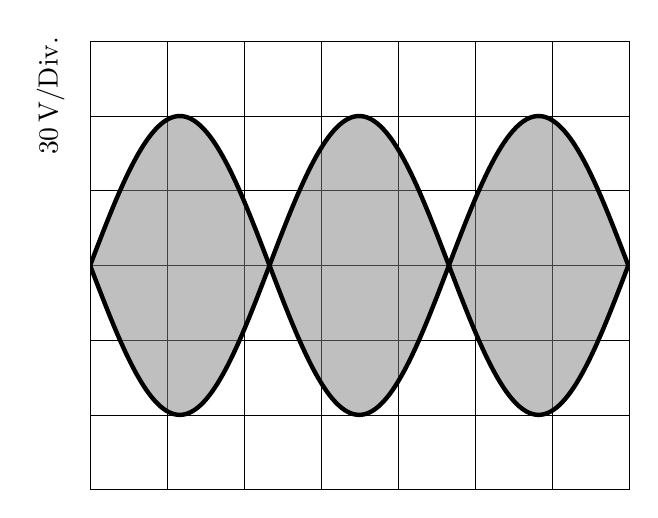
\begin{tikzpicture}
    \pgfplotsset{samples=200}
    \begin{axis}[
        ticks=none,
        xmin =  0,
        ymin = -3,
        xmax =  7,
        ymax =  3,
        domain = 0:7,
        grid=both,
        grid style={line width=.1pt, draw=black},
        major grid style={line width=.2pt,draw=black},
        xtick = {0,1,2,3,4,5,6,7},
        ytick = {-3,-2,-1,0,1,2,3},
        thick,
        smooth,
        no markers]
        \addplot+[name path=A,ultra thick, black] { 2*sin(deg(x*1.35)-0)+0};
        \addplot+[name path=B,ultra thick, black] {-2*sin(deg(x*1.35)-0)+0};
        \addplot[gray, opacity=0.5] fill between[of=A and B];
    \end{axis}
    \node[rotate=90] at (-0.5,5) {30\,V/Div.};
\end{tikzpicture}
\end{document}
